%%%%%%%%%%%%%%%%%%%%%%%%%%%%%%%%%%%%%%%%%%%%%%%%%%%%%%%%%%%%%%%%%%%%%%%%
\def\stitle{Wiederholung Typumwandlung}
\section{\stitle}\label{K:wdh}
\begin{frame}
  \frametitle{\kap. Wiederholung}%
\tableofcontents[current]
\end{frame}

%%%%%%%%%%%%%%%%%%%%%%%%%%%%%%%%%%%%%%%%%%%%%%%%%%%%%%%%%%%%%%%%%%%%%%%%
\begin{frame}[fragile]%
  \frametitle{\kap. \stitle}%
\medskip

Überführung von Datentypen ohne Verlust entlang der Pfeilrichtung.
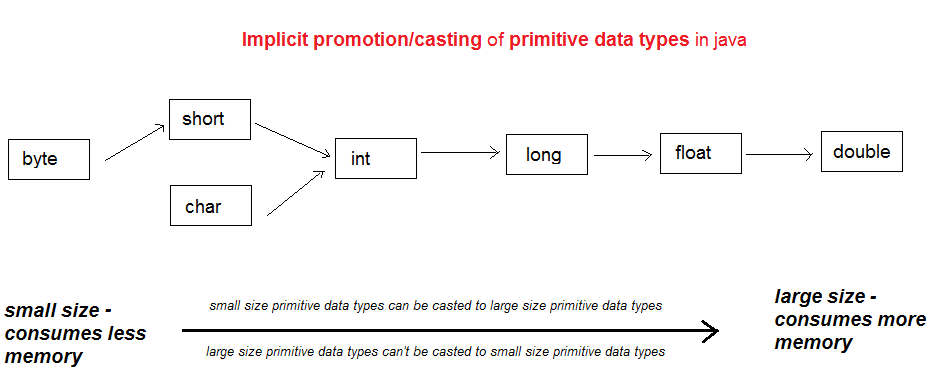
\includegraphics[width=12cm]{\getexercisefolder/cast.png}

\begin{lstlisting}[style=java, frame=single]
double a = 9.6;
int n = (int) a; // Verlust von Information (n=9)
\end{lstlisting}
\end{frame}



%%%%%%%%%%%%%%%%%%%%%%%%%%%%%%%%%%%%%%%%%%%%%%%%%%%%%%%%%%%%%%%%%%%%%%%%
\begin{frame}[fragile]%
  \frametitle{\kap. \stitle}%
\medskip

Allgemein \code{(Datentyp)(Ausdruck)}.
\lstinputlisting[style=JAVAlines]{\getexercisefolder/Typumwandlung.java}

\end{frame}
